\documentclass{llncs}

\usepackage{hyperref} 
\usepackage{subfigure}
\usepackage{graphicx}
\usepackage{url}
\usepackage{times}
\usepackage{multirow}
\usepackage{amsmath}
\usepackage{amssymb}
\usepackage{xspace}
\usepackage{epsfig}
\usepackage{todonotes}
\usepackage{array}
\usepackage{caption}
\usepackage{graphicx}
\usepackage{mathtools}
\usepackage{algorithm}
\usepackage{algpseudocode}
\usepackage{algorithmicx}
\usepackage{todonotes}
\usepackage[printonlyused]{acronym}
\usepackage{microtype}
\usepackage{cleveref}
\usepackage{xcolor}
\usepackage{caption} 
\captionsetup[table]{skip=10pt}


\title{Computational Intelligence in Games}%
\author{Julian Blank, Frederick Sander}%
\institute{Otto-von-Guericke-University Magdeburg, Germany \\ julian.blank@st.ovgu.de \\ frederick.sander@st.ovgu.de}

\hypersetup{
    colorlinks,
    linkcolor={red!50!black},
    citecolor={blue!50!black},
    urlcolor={blue!80!black},
    pdftitle = {\@title},
    pdfauthor = {\@author}
}




\newcommand{\keywords}[1]{\par\addvspace\baselineskip\noindent\keywordname\enspace\ignorespaces#1}
\newcommand{\vect}[1]{\boldsymbol{#1}}
\providecommand{\e}[1]{\ensuremath{\times 10^{#1}}}
\DeclareMathOperator*{\argmax}{arg\,max}

\hyphenation{proving}
\setcounter{secnumdepth}{5}




\begin{document}


%\setcounter{tocdepth}{1}
%\listoftodos



\mainmatter
\maketitle



\begin{abstract}
\todo{
Summarize the paper in a paragraph of two. It should contain at least 70 and at most 150 words. You should motivate the research done, give some details about the experiments run and briefly mention the most important findings. 
}
\end{abstract}



\section{Introduction} 
\label{sec:intro}


The game industry was growing over the past years~\cite{gartner}. Therefore 
constructing good game artificial intelligences (AI) comes more and more important.
Normally a game AI is created for one specific game. Often if a human plays against
enemies there are different levels of difficulties that could adjusted.
Our aim of the course "Computational Intelligence in Games"~\footnote{http://is.cs.ovgu.de/Courses/Team+Projects/Computational+Intelligence+in+Games.html} at the Otto-von-Guericke-University Magdeburg in Germany~\footnote{http://www.ovgu.de/} was
to evaluate three different approaches on the General Video Game AI Competition~\footnote{http://www.gvgai.net/}.
The task is to create a game AI that play unknown games as best as possible. The agent can observe the
whole grid with game objects that move. Besides he gets information of all the collision that happened.
Moreover the agent has 40 ms for each game step to act. All actions - depending on the game - are  LEFT, UP, RIGHT, DOWN, USE and NIL.
To find the best action the agent could simulate steps and so predict the next state.
But there is uncertainty because the game objects move randomly.

All this facts form a difficult problem to solve. The agent should play tight to win the most games as fast as possible. 
Also the advancement has to be general because he should dynamically find out what is the target of the current game.

There are different approach to create an game AI. Therefore we first outline our literature review and explain after that
the background of the approaches. The theory could not always be implemented like it was proposed because it has to
fit the requirements of the games. For this reason we explain at the chapter 4 the details of our implementations.
Then we evaluate first the best setting of each approach. Thereafter the best agents of them are compared and the
winner comes out ahead.








\section{Literature Review} \label{sec:lit}
\todo{
Perform a literature review: What has been done before in this field? What is the main technique/s used in the paper, and what has it/they been used for in the literature before? Give references to the most relevant work published. Example: ~\cite{BrowneMCTSurvey}.
}

The field of Computational Intelligence in Games, blow CIG, is very wide and There is a lot of work related  to this theme. We are dealing with the topic of General Video Game Playing, below GVGP, which belongs to the umbrella term CIG...


\section{Background} 
\label{sec:back}

There are several basic approaches to write an artificial intelligence (AI) for a game. In this project we were forced to investigate different ideas at three different research areas: heuristic based search, reinforcement learning and nature inspired algorithm. 
Of course there is an overlap between these approaches. All of them try to find the next best step for the agent by iterating through a search tree. This is build in base of all possible game steps that could done by the agent.
One naive approach of iterating through the whole search tree is not possible, because there is a time limitation.
Generally this leads to solve the trade-off between iterating similar to a breadth-first or depth-first search.
The heuristic approach forces the second by using a estimation function for looking many steps ahead.


\subsection{Heuristic Based Search} 

A heuristic is used to evaluate a game state by putting several facts into one number. When we have to decide which current active branch of a search tree should be iterated this score might help us. 
One common idea to estimate the distance to the target is the manhatten distance~\cite{distance_metrics}. 

In a two dimensional space the manhatten distance is calculated by

\begin{equation}
dist(u,v) = |x_{1} - x_{2}| + |y_{1} - y_{2}|
\end{equation}

adding the absolute value of the difference for the $x$ and the $y$ axis. The input consists always of the points that have one value for each dimension. This could be extended for a n-dimensional space as well. When thinking of a way at a grid this is always a path with one rectangle waypoint (see Figure ~\ref{fig:manhatten}).

\begin{figure}
\centering
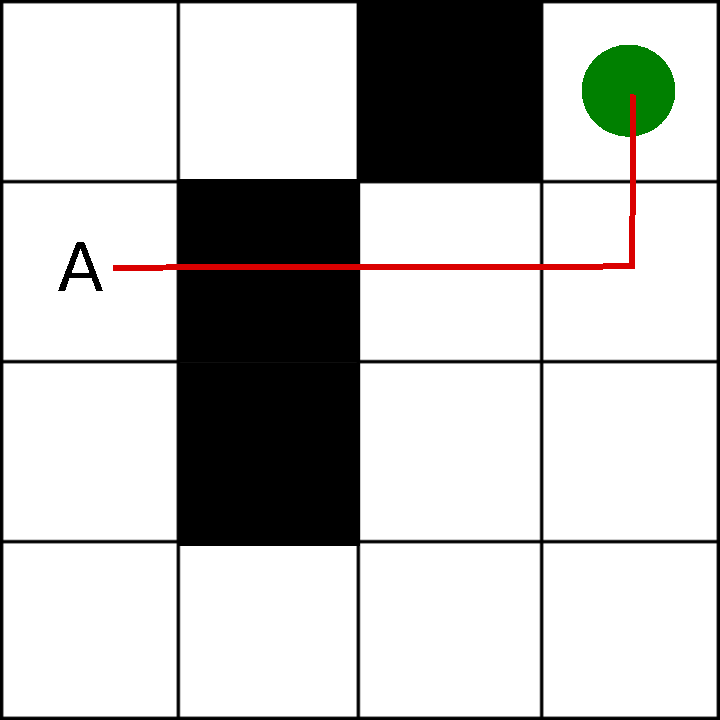
\includegraphics[scale=0.3]{images/manhatten.pdf}
\caption{Manhatten distance}
\label{fig:manhatten}
\end{figure}



\subsubsection{Greedy}

Greedy-algorithms are a whole class of algorithms and strategies. All of them follow a specific scheme/rule. They are iterative and choose in every step the state with the best reward. The state is in most cases a node which represents the state of the algorithm. The advantage of greedy algorithms is that they are very fast but on the other hand they are not optimal they often only find a local optima and not the global one. The advantage and disadvantage is caused by the greedy approach.  

\subsubsection{One Step Lookahead}

One step lookahead is a very simple tree search algorithm which follows the greedy approach. The actual state is the root node. From this node we only look one step ahead to all nodes which are connected by one edge and compute a heuristic value or another kind of reward value for these nodes. 

\begin{figure}
\centering
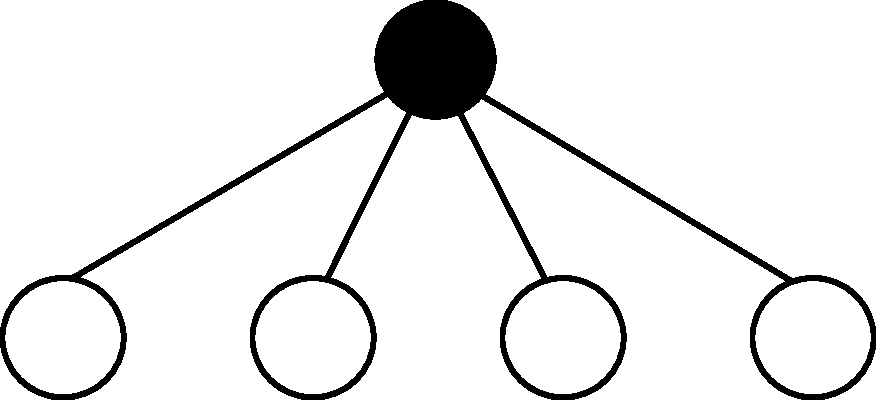
\includegraphics[scale=0.3]{images/onestep_lookahead.pdf}
\caption{Search tree for One Step Lookahead}
\label{fig:onestep}
\end{figure}


After that the algorithm terminates and we pick the node with the best value.

\subsubsection{AStar}

The A* tree search algorithm is a modification of the dijkstra algorithm and also belongs to the class of greedy algorithms. The Algorithm finds the shortest path between two nodes. In difference to normal greedy algorithms A* is a optimal algorithm, it finds a solution when a solution exists (in this case the shortest path). The algorithm uses a heuristic to estimate the shortest path. The value f(x) of a node N is the sum of its heuristic value h(x) and the costs from the start-node to N g(x).

\begin{equation}
f(x)=h(x)+g(x)
\end{equation}


A* contains two sets of nodes, the openlist and the closedlist. In every step of the algorithm the Node N with the lowest f(x) value in the openlist is put on the closedlist and all its connected nodes, which are not in the closedlist, are put in the openlist (with reference to their fahter N). If a connected node is already in the closedlist but the new generated value f'(x) is lower than f(x) then f(x) will be replaced by f'(x) and the new father-reference is N. The openlist contains all the nodes to which the path is already known and which can be checked in the next step, the closedlist contains every visited and checked node. When the actual node is the goal-node, the algorithm terminates. To generate the path, the algorithm goes back from the goal-node to the start node (guided by the father-references). 

\subsection{Reinforcement learning} 
 
Reinforcement learning, below RL, is a field in Machine learning which is a section of Artificial Intelligence. RL methods are mostly used by agents in an environment called Markov decision process, below MDP. MDP is a mathematical description of decision processes. They have different states S and some actions A which are available in the actual state. Every timestep the agent chooses an action $a$ and the process switches from state $s_a$ to $s_n$. The probability to go over form a state S to another state S' by any action A can be described as

\begin{equation}
	G: S*S*A \rightarrow [0,1] 
\end{equation}

and the reward given to the agent can be described by this:

\begin{equation}
	R: S*S*A \rightarrow \mathbb{R}
\end{equation}

So that

\begin{equation}
	(s_a, s_n, a) \rightarrow p(s_n|s_a, a)
\end{equation}

would describe the probability $p$ to go over in the state $s_n$, given the actual state $s_a$ and the choosen action $a$ and 

\begin{equation}
	(s_a, s_n, a) \rightarrow r
\end{equation}

shows its corresponding reward.  


In differ to other learn methods and approaches like the (semi)supervised learning, RL algorithms never use information which they do not figured out themselves, so no correct samples were given to the algorithm. The only information is the reward given to the agent and some additional information like heuristic values, depending of the specific algorithm. 
A big problem problem in RL is the conflict between exploration of new and unvisited areas of the solution room and exploitation which is the improvement of already found solutions.
...
\subsubsection{Monte Carlo Tree Search} 

Monte Carlo Tree Search, below MCTS, is a class of RL algorithms. It is the most important concept in this paper. MCTS needs a tree of nodes which represent the different states, the edges represent the actions used by the agent to get to this node. The MCTS algorithm traverses to this tree and expands it. To find the global optimum a good balancing ratio between exploration and exploitation is required. 

[maybe picture from his paper and pseudocode]

The general MCTS algorithm has four steps, selection, expansion, simulation and backpropagation. In the selection the algorithm starts at  



\subsection{Nature inspired} 
The nature is solving problems by applying different approaches instinctively. 

\subsubsection{Neural nets} 
Our brain solves many problems that could not be solved by algorithms yet. Many researcher tries to explore the process of the human brain. Neural networks tries to model the nervous system and to adapt all the processes~\cite{nn_intro}. The neurons are modeled as \textit{threshold logic units} (TLU) that consists of several input values $x_1$ to $x_n$ and one output value $y$~\cite{ci_kruse}. 


\begin{figure}
\centering
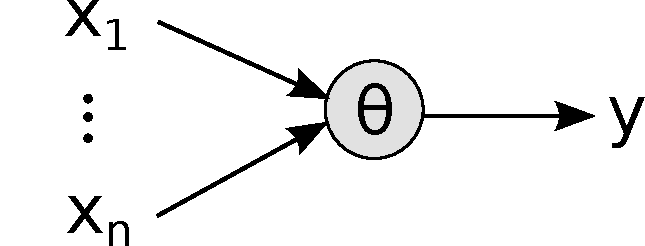
\includegraphics[scale=0.3]{images/tlu.pdf}
\caption{threshold logic units ~\cite{ci_kruse}}
\label{fig:tlu}
\end{figure}


For computing the output value is always for every input value one weight $w_i$ and the threshold $\theta$. The formula 

\begin{equation}
    y = 
\begin{dcases}
    1, & \text{if } \sum_{i=1}^n w_{i} x_{i} \geq \theta \text{,} \\
    0, & \text{otherwise.}
\end{dcases}
\end{equation}

is used to calculate the output $y$ that is either 0 or 1.
Normally the input and the output is given and the weights has to be learned. With only one TLU there only linear separable spaces could be learned perfectly.
To solve that problem there is the possibility to create a network of TLU's and map that problem to a higher dimensional space~\cite{ci_kruse}.




\subsubsection{Evolutionary algorithm} 
An \textit{Evolutionary Algorithm} (EA) tries to use the biological behavior of the population~\cite{evo}. 


\begin{algorithm}
\caption{Evolutionary Algorithm~\cite{evo}}
\label{alg:evo}
\begin{algorithmic}
\State \emph{Initialize} Population with random candidate solutions;
\State \emph{Evaluate} each candidate;
\While{Termination condition not satisfied} 
\State \emph{Select} parents;
\State \emph{Recombine} pairs of parents;
\State \emph{Mutate} the resulting offspring;
\State \emph{Evaluate} new candidates;
\State \emph{Select} individuals for the next generation;
\EndWhile
\end{algorithmic}
\end{algorithm}




\subsubsection{Pheromones} 




\section{Techniques Implemented} 
\label{sec:exp}

After explaining the theory of several approaches we now describe our implementations. The proposed algorithm are not always fitting to 
the principle of the games or has a lot of parameter that has to be adjusted to have good results. We first point out same basic strategies
for example staying alive.


\subsection{Stay Alive} 

We implemented two different Stay Alive Agents that has the aim just to act safe and hopefully randomly win the game.
Even if there is the possibility to simulation an action, there is all the time an uncertainty. All objects of the games in our competition
could - but has not - to act randomly. If we are using the \textit{advance} function that allows us to simulate one step that just
one possible state of the future. This implies even if we are not dying at our simulation we could die at the real game.

One approach is to simulate the next action $n$ times. If the agent does not die for this simulations the next action should be safe.
The problem is to set a good value for $n$. If the value is to large not all the possible actions could be tested. Otherwise 
if it's to small the probability that it's even unsafe grows.
From the resulting safe action set there could be randomly choosen the final action.

\begin{figure}
\centering
\begin{minipage}{.5\textwidth}
  \centering
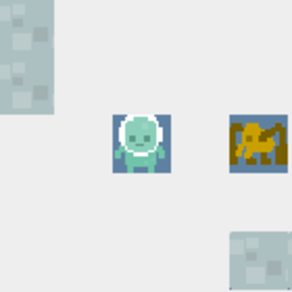
\includegraphics[scale=0.8]{images/safe.pdf}
\caption{Advancing safe actions}
\label{fig:safe}
\end{minipage}%
\begin{minipage}{.5\textwidth}
\centering
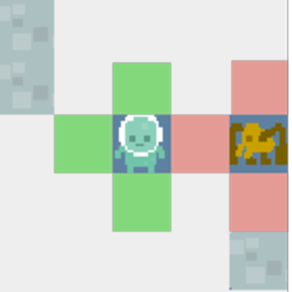
\includegraphics[scale=0.8]{images/safe_grid.pdf}
\caption{Grid search for safe actions}
\label{fig:safe_grid}
\end{minipage}
\end{figure}



Suppose there is a game situation like in~\cref{fig:safe} the action \textit{RIGHT} is definitely unsafe what 
should after an amount of $n$-action be clear.

Another idea is to analyse the grid around the agent. Assume that each enemy could only move one field at the grid
at one game step there is a $5x5$ grid that needs to be analyzed. If an enemy at this grid exists one action is
maybe unsafe. If not the enemy won't die for sure.




At the~\cref{fig:safe_grid} you can see the action that could be excluded without doing any simulation at the game.
The possible next fields (excluded the current position if agent does nothing) are marked green. The possible positions
of the enemy are red. The action RIGHT is by using the grid search unsafe. 
At first glance it looks faster and better to only look at the grid, but there might be some problems for unknown games:

\begin{itemize}
  \item One problem is to classify the game objects at the grid. The grid search is only good if we know that this objects represents an enemy. Otherwise
  we also classify walls as unsafe.
  \item Not every enemy could move to all directions. have a look at the figure 
\end{itemize}



\subsection{Heuristic based} 
 
If the action is only safe the will be the problem that no target is forced because the selection happens randomly.
Therefore a heuristic is used to evaluate one state and get a score. When we previously know the game
that would be one good approach. But whenever the game is unknown the result will be completely different.
One heuristic could be very good for example where the agent could kill an enemy. But if in another game
the enemy will kill us the heuristic let commit us suicide.

To fix that we had two different ideas. On the one hand we could implement a dynamic heuristic that is changing over time
and learn from the environment. On the other hand there could be a third instance that we called \textit{Explorer} 
that is learning from the environment and creating a knowledge-base. 
To use this idea always for further approaches we forced on the second idea.

During the construction time the agent only explores the environment. 
First of all he creates a list with all interesting targets that exists at the level. For all of them he sends pheromones into the grid
and simulate until the agent dies. 
For all the simulation there is a global class the \textit{Simulator} that automatically make inferences from the observations.
The knowledge base is the environment class that contains information to blocking, scoring, winning and loosing game objects (sprites).
This two classes follows the singleton pattern and could be created by using the factory (cf.~\cref{fig:sim_classes}).
Additional information that you can see at the figure is the game detection that is explained later and the field tracker that keeps 
information about all fields at the grid and how often the agent visited each one.

\begin{figure}
\centering
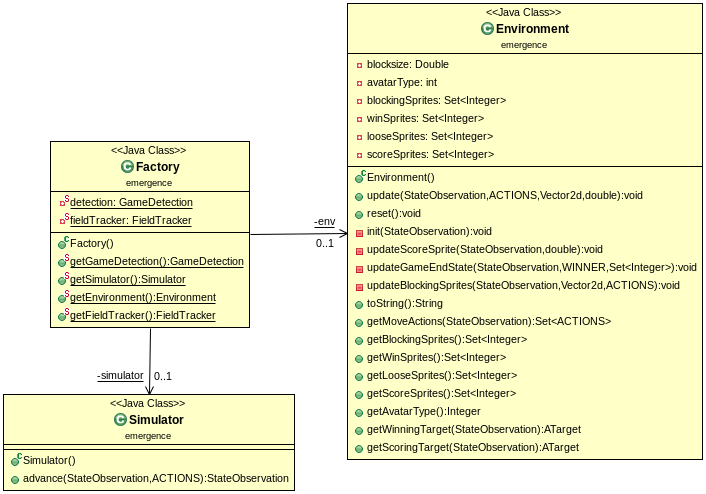
\includegraphics[scale=0.5]{images/classes.png}
\caption{Class diagram of the simulator and environment structure}
\label{fig:sim_classes}
\end{figure}


When the explorer find the winning or scoring objects a heuristic is initialized. We used a heuristic with that 
calculates the distance to one target by using the mannhatten distance. To reach this target we use an astar 
algorithm with three modifications.

Every game step the astar algorithm is executed from scratch even if we found the target in the last iteration.
We use an safety approach for the first action to ensure the next action we maybe choose is safe. For that we
use the principle of the stay alive agent. The astar algorithm needs to hold all the states in memory.
This leads to a very fast growing open list with a lot of states. We introduce a \textit{maxStates} variable. 
Whenever the open list of the astar algorithm is larger than this variable the list is cut in a half.
Additionally we use for our simulations the simulator and use the knowledge base. Normally all children of
a state are added to the open list. We only add all the children to the list of that we assume we will get a 
new position. Since we know from the Environment class which objects are blocking, we could use that information
for a smarter iteration.


\subsection{MCTS Tree} 

The theory of MCTS-treesearch is described in section 3. The standard approach was modified to fit our problem. The whole MCTS algorithm is computed in the class \textit{MCTSStrategy} which is used by the \textit{MCTSAgent} and the \textit{MCTSHeuristicAgent}.

\subsubsection{tree policy}
Our tree policy iterates trough the tree, starting at the root node. When a node is not fully expanded, a randomly chosen children node is generated. We tried out some other ways to chose the children, but random selection worked best. If we reach a fully expanded node the tree policy uses a modified UCT formula

\begin{equation}
 	UCT = \frac{c.Q}{c.V + ep * r} + \sqrt{\frac{\ln (n.V+1)}{c.V}}
\end{equation} 

to chose the children node. Where \textit{n} is the node and \textit{c} the actual children. \textit{Q} is the reward of a node and \textit{V} the number of visits, more precise the number of times the tree policy had chosen this node. The exploitation term is computetd by dividing the reward of the child by the number of vistis and a random factor to avoid divisions by zero. This term is big for nodes whose reward is high on average.
When the childs number of visits are small in comparison to the others, the second term (exploration) will be big. We tried out some other varaints and factors but this solution has the best results. It is very close to the original UCT formua (see section 3).   

\subsubsection{default policy \& backpropagation}

The default policy tries to figure out how good the given node from the tree policy is. To do that, a simulation with the correspond state observation and random actions is done. It is repeated until the hypotethical level of the simulated node reaches the before defined maximum (maximal depth of the tree). At the beginning, when the tree is small, more simulations are executed. Later, when we have already grown our tree, only a few simulations are executed. We chose this approach because at the begnning we have no information about the node and its neighbourhood so we have to compute more simulations....
When the simuation is finished a reward is generated from the last state observation by the delta heuristic which is descibed later. The win, loss and score were considered.
The backpropagation iterates from the node which was expanded by the tree policy to the root, guided by the father references of every node. To every visited node the reward is added and weigthed with a before specified value.

\subsubsection{rolling horizon}

The implementation of a rolling horion working on it......

\begin{itemize}
  \item tree policy
  \item default policy
  \item act choosig -> most visited node
\end{itemize}
























\subsection{Evolutionary algorithm} 

The theory of the evolution has to be mapped to the gaming problem. Each candidate of our population is
a list of actions that could be executed. To evaluate the fitness of a candidate we are using the
simulation function that is provided by the game. 
The score

\begin{equation}
s = \sum_{t=0}^n (H(s_t) - H(s_{t-1}))
\end{equation}

is calculated by using the function

\begin{equation}
    H(s_i, s_{i-1}) = 
\begin{dcases}
    10, & \text{if isWinner}  \\
    -10, & \text{if isLooser}  \\
    score(s_i) - score(s_{i-1}), & \text{otherwise.}
\end{dcases}
\end{equation}

what we called delta heuristic function.

We implemented two very naive operations on the pool. The crossover is done by
select for 50 \% the action of the first or the second individual (cf.~\cref{fig:crossover}).

\begin{figure}[H]
\centering
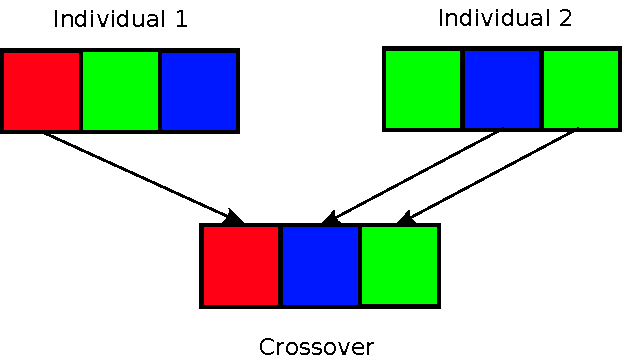
\includegraphics[scale=0.6]{images/crossover.pdf}
\caption{Crossover of an individual}
\label{fig:crossover}
\end{figure}

The mutation is implemented by doing an crossover with an random individual.
We fixed for all evaluations runs the mutation probability to $0.7$ which implies a crossover 
probability of $0.3$.

We had several problems with the limited time for the evolution.
For that we want to have always a good starting pool and use our information from the last
game step. All candidates from the last final pool of the last game step are used for the initialization.


\begin{figure}[H]
\centering
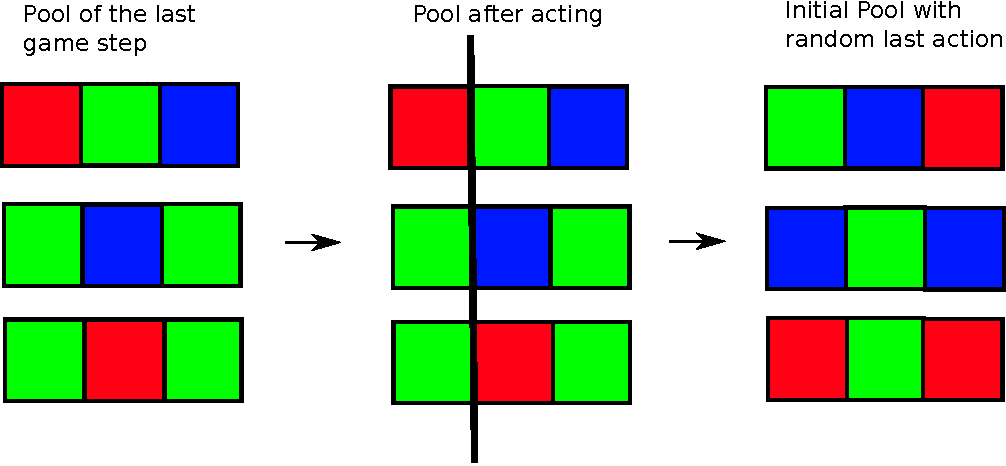
\includegraphics[scale=0.6]{images/sliding_window.pdf}
\caption{Sliding Window}
\label{fig:sliding_window}
\end{figure}

For that we use the principle of a sliding window (cf.~\cref{fig:sliding_window}). The first
action from the last pool is removed because the agent was acting like this at the last game step. Then
to keep the action length fix there is added one random action to the action path.
By using that principle we are not throwing our last simulations away.

There is also the problem that for different games the simulation time differs. If we have many game objects that 
need to be updated and checked for collision, the simulation time increases.
But to find a good value for the pool size we need to know the calculation time.
As a fix for this we introduced the adaptive path length that reduces or increases the actions
of every individual.
For that we forced to get always the fourth generation. On the one hand if we stay for example at the initial
pool because the evaluation takes to long we will reduce the path length. On the other hand if the agents acts like 
the seventh generation we force to have a long time planing by increasing the path length.

Another problem that we tried to fix is to avoid situations where no individual has a positive score or many has a score of zero. That means each 
candidate is not gaining points. Our first implementations solved such a tie randomly. 
The randomness could be disabled by using a heuristic. If we would always use the same heuristic that would not work
for all the games because they have different aims. 
So we used a heuristic switch after $n$ time steps to have also a long time planing strategy.


  
  
\subsection{Game Detection} 
  
Another technique we have implemented is a detection of a known game. We know the 10 games from the test-set and the 10 games from the validation-set, the 10 test-set games are unknown. The Goal of the Gamedetection is to improve the score and the number of wins in the two known game-sets without decreasing the score and the number of wins in the unknown test-set. To do that, the standard parameters of the Algorithm are used when no game is detected, otherwise the optimal parameters for this game are used. These parameters we figured out for some difficult games in which the standard parameters give bad results. To detect a game we generate a String of all Objects (npc, movable, immovable, ect...) and store the Hash value of this String. All the hashes from the known games are stored, in a running Game we generate another String of these Objects and compare the generated hash value to the stored ones. 

\section{Experimental Study} 
\label{sec:exp}

\todo{Detail the experimental setup used to test the different algorithms. Present the results in an understandable manner (graphics, tables, etc.). Draw conclusions about what things worked (and why) and which didn't (and why).  \ldots}
\todo{maybe the wrong place for this paragraph, introduction and describes the test environment}

To test how well the implemented algorithms work we executed the games a lot of times. We have the 20 games from the trainings- and validationset to test the algorithms. We had no acces to the origial test set. First of all we want to compare the 3 different controllers with each other but the several different parameters we can change in the controllers are also interesting.
To test a agent we ran 1000 Games, one game 50 times and one single level 10 times. The following machine was used to run all of the simulations:

\begin{table}
\center
\begin{tabular}{ll} 
\textbf{CPU} & 4x Inted(R) Core(TM) i5-4210U CPU @ 1.70Ghz \\ \hline
\textbf{Memory} & 8 GB DDR3 L \\  \hline
\textbf{Operating System} \mbox{   } & Ubuntu 14.04.1 LTS \\  \hline
\textbf{Java Version} &  \\  
\end{tabular}
\caption{experiment setup}
\end{table}


Only this machine was used because with the same agent and parameters we achived on different machines very different results. The computational power from the cpu was ?ausschlaggebend for our choice. The reason of the different results is that the agent every gametick only has 40ms to return an action. The results from a powerful CPU were better and more stable (the derivation was ?kleiner) than the results from an ?schlechter CPU. To evaluate the results we stored them in csv files and generated tables.

For every evaluation is first of all a table with all there parameter settings. Additionally there are the average winning rate and the standard deviation listed.
All the results are also visualized by boxplots. There you can see the minimum and maximum average wins overall iterations. Furthermore the blue rectangle shows 
the qartile values. The red line in the middle is the median and the blue dot is the mean (average wins).
Do not mix quartiles with the standard deviation that is something completely different.

In the following sections each of the approaches is evaluated. 

\todo{combinations really failed. explain it.}
\todo{why we use this parameters??? something is missing...why not an exhaustive search for finding the best parameter..no time? 
to less computational power...}

\subsection{Heuristic based Algorithm} 

The heuristic based algorithm has several parameter that changes the behaviour of the agent (cf.~\cref{tbl:heur}).
Firstly we just changed the maximal states field that provides a limit for saved states at
the AStar algorithm. As you can see the average winning rate increases by changing to a higher maximal states limit up to 20.
But if the variable is set to 25 we had a worse result. This might be that if this value is to low the target is not found 
by the AStar algorithm. Moreover if it is to large to many states are saved and we get trouble with the memory or the
garbage collector.


\begin{table}[htbp]
\center
\begin{tabular}{*9c}  \hline
\multicolumn{1}{p{1cm}}{\centering ID} & 
\multicolumn{1}{p{2cm}}{\centering Max.\\ States} & 
\multicolumn{1}{p{2cm}}{\centering Safety\\ Strategy} & 
\multicolumn{1}{p{2cm}}{\centering Safety\\ Iterations} & 
\multicolumn{1}{p{1cm}}{\centering Avg\\ Wins	} & 
\multicolumn{1}{p{1cm}}{\centering Std of Wins} \\ \hline
1 & 5 & SafetyAdvance & 5 & 0.517 & 0.026 \\ \hline
2 & 15 & SafetyAdvance & 5 & 0.529 & 0.020\\ \hline
\textbf{3} & \textbf{20} & \textbf{SafetyAdvance} & \textbf{5} & \textbf{0.532} & \textbf{0.027} \\ \hline
4 & 25 & SafetyAdvance & 5 & 0.521 & 0.019 \\ \hline
5 & 20 & SafetyGridSearch & - & 0.498 & 0.024 \\ \hline
6 & 20 & SafetyIntelligent & 5 & 0.527 & 0.018 \\ \hline
\end{tabular}
\caption{results of the \ac{HR} algorithms}
\label{tbl:heur}
\end{table}
\begin{figure}[H]
\centering
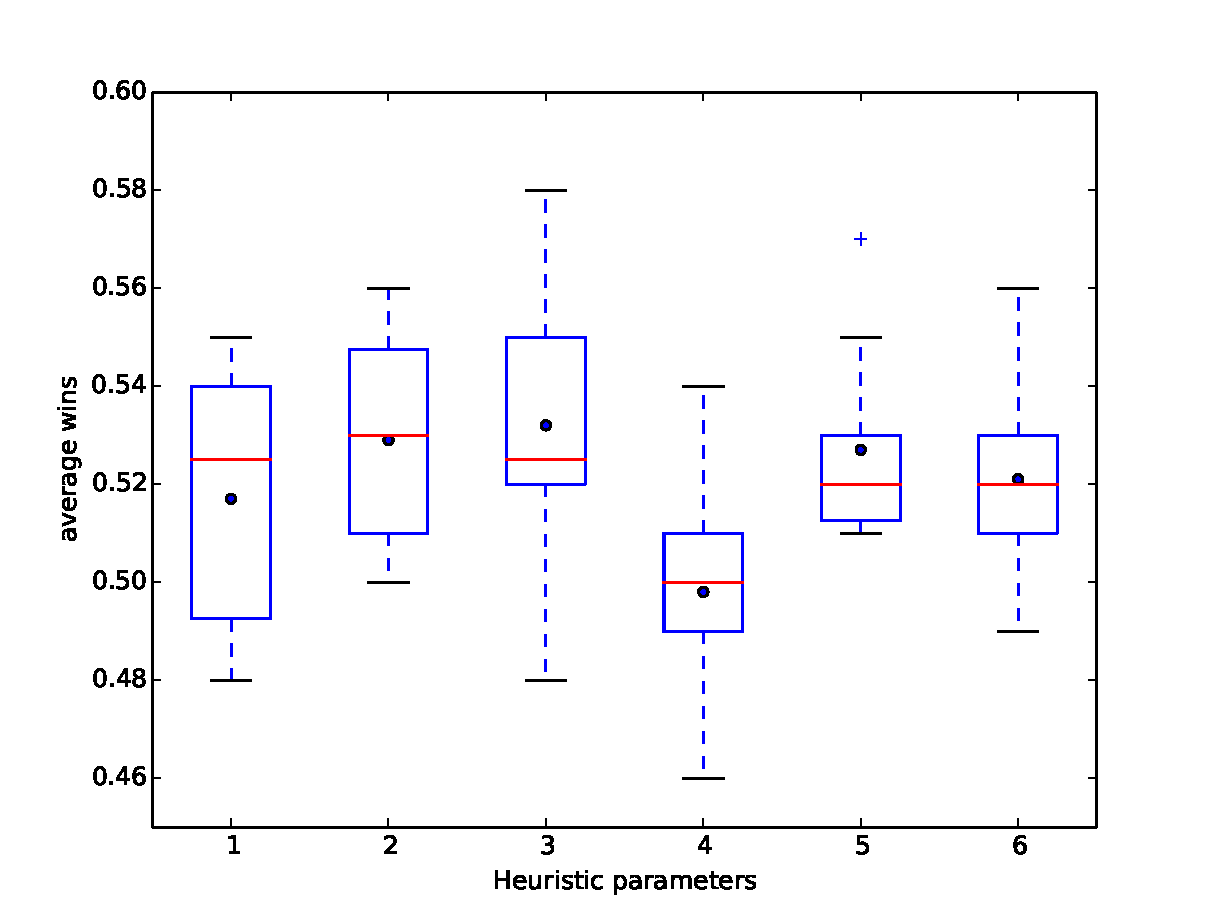
\includegraphics[scale=0.5]{images/eval_heur.pdf}
\caption{boxplot of the heuristic based algorithms}
\label{fig:eval_heur}
\end{figure}

After that we tried to change the safety strategy to the grid and the intelligent search. Both results
are worse than the SafetyAdvance Strategy. Since the SafeGridSearch highly depends on the Explorer and the
classification of the object this might be the cause.
With the SafetyIntelligent we got no further improvement but it is nearly good as the SafetyAdvance approach.

The boxplot (cf.~\cref{fig:eval_heur}) visualizes the quartiles. The best parameter setup has also the largest
quartile range. When you look at the table also the largest standard deviation (which doesn't have to be the same).
If the target is not found the agent is staying alive. The risk of a longer search to reach a simulation state
that collides with the target could be the reason for the higher variance of the results.



\subsection{MCTS} 
We also tried to combine several approaches for example using the heuristic explorer 
for a better mcts iteration. 

\begin{table}[H]
\center
\begin{tabular}{*9c}  \hline
\multicolumn{1}{p{1cm}}{\centering ID} & 
\multicolumn{1}{p{2cm}}{\centering rolling \\ Horizon} & 
\multicolumn{1}{p{2cm}}{\centering maximal \\ TreeDepth} & 
\multicolumn{1}{p{1.5cm}}{\centering gamma} & 
\multicolumn{1}{p{2cm}}{\centering Avg\\ Wins	} & 
\multicolumn{1}{p{2cm}}{\centering Std of Wins} \\ \hline
1 & 0 & 10 & 1 & 0.383 & 0.033 \\ \hline
2 & 1 & 10 & 0.9 & 0.401 & 0.026 \\ \hline
3 & 1 & 3 & 1 & 0.416 & 0.014\\ \hline
4 & 1 & 5 & 1 & 0.402 & 0.030 \\ \hline
\textbf{5} & \textbf{1} & \textbf{7} & \textbf{1} & \textbf{0.422} & \textbf{0.033} \\ \hline
6 & 1 & 10 & 1 & 0.412 & 0.025 \\ \hline
7 & 1 & 15 & 1 & 0.394 & 0.014\\ \hline
8 & 1 & 20 & 1 & 0.395 & 0.025 \\ \hline
9 & 1 & 25 & 1 & 0.384 & 0.026 \\ \hline
\end{tabular}
\label{mcts_result}
\caption{\ac{MCTS} result}
\end{table}

\begin{figure}[H]
\centering
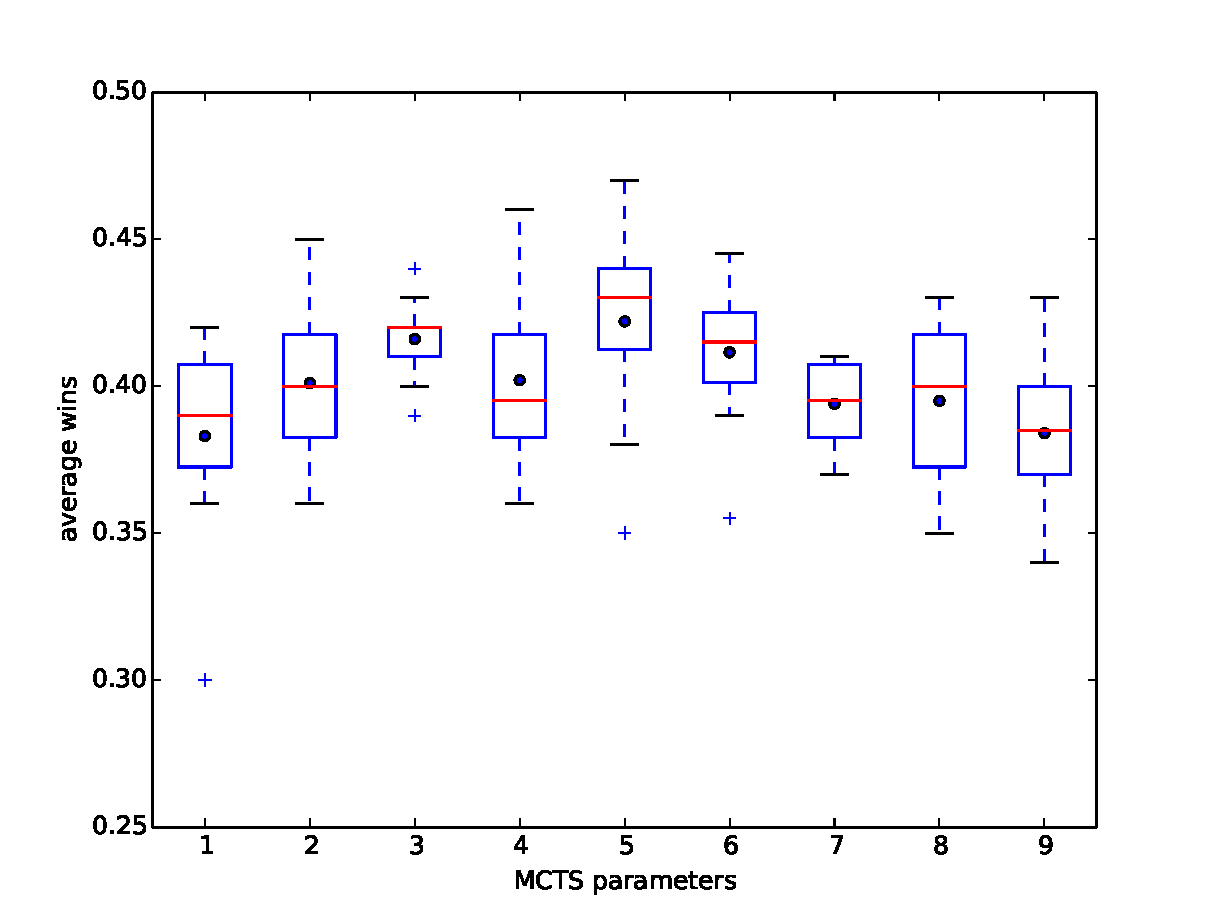
\includegraphics[scale=0.6]{images/eval_mcts.pdf}
\caption{boxplot of the \ac{MCTS} algorithm}
\label{fig:eval_evo}
\end{figure}


\subsection{Evolutionary Algorithm} 

For the evolutionary algorithm we had a set up with different parameters.

\begin{table}[H]
\center
\begin{tabular}{*9c}  \hline
\multicolumn{1}{p{1cm}}{\centering ID} & 
\multicolumn{1}{p{2cm}}{\centering Safety\\ Iterations} & 
\multicolumn{1}{p{1cm}}{\centering Path Length} & 
\multicolumn{1}{p{1cm}}{\centering Size of\\ Pop.} & 
\multicolumn{1}{p{1cm}}{\centering Fittest\\ Pop.} & 
\multicolumn{1}{p{1cm}}{\centering Dyn. Path\\ Length} & 
\multicolumn{1}{p{1cm}}{\centering Min. Gen.} & 
\multicolumn{1}{p{1cm}}{\centering Avg \\ Wins	} & 
\multicolumn{1}{p{1cm}}{\centering Std of Wins} \\ \hline
1 & 2 & 6 & 14 & 5 & no & - & 0.459 & 0.023 \\ \hline
2 & 4 & 6 & 10 & 4 & no & - & 0.458 & 0.024 \\ \hline
3 & 5 & 4 & 14 & 5 & no & - & 0.466 & 0.028 \\ \hline
4 & 5 & 6 & 10 & 5 & no & - & 0.459 & 0.032 \\ \hline
5 & 5 & 6 & 13 & 4 & yes & 5 & 0.451 & 0.041 \\ \hline
6 & 5 & 6 & 14 & 3 & no & - & 0.471 & 0.018 \\ \hline
7 & 5 & 6 & 14 & 5 & no & - & 0.461 & 0.025 \\ \hline
\textbf{8} & \textbf{5} & \textbf{6} & \textbf{14} & \textbf{5} & \textbf{yes} & \textbf{2} & \textbf{0.479} & 0.021 \\ \hline
9 & 5 & 6 & 14 & 5 & yes & 4 & 0.463 & 0.027 \\ \hline
10 & 5 & 6 & 14 & 5 & yes & 6 & 0.449 & 0.041 \\ \hline
11 & 5 & 6 & 14 & 7 & no & - & 0.474 & 0.028 \\ \hline
12 & 5 & 6 & 18 & 5 & no & - & 0.462 & 0.035 \\ \hline
13 & 5 & 8 & 14 & 5 & no & - & 0.453 & 0.029 \\ \hline
14 & 8 & 6 & 14 & 5 & no & - & 0.477 & 0.022 \\ \hline
\end{tabular}
\label{ea_result}
\caption{results of the \ac{EA} algorithms}
\end{table}



\begin{figure}[H]
\centering
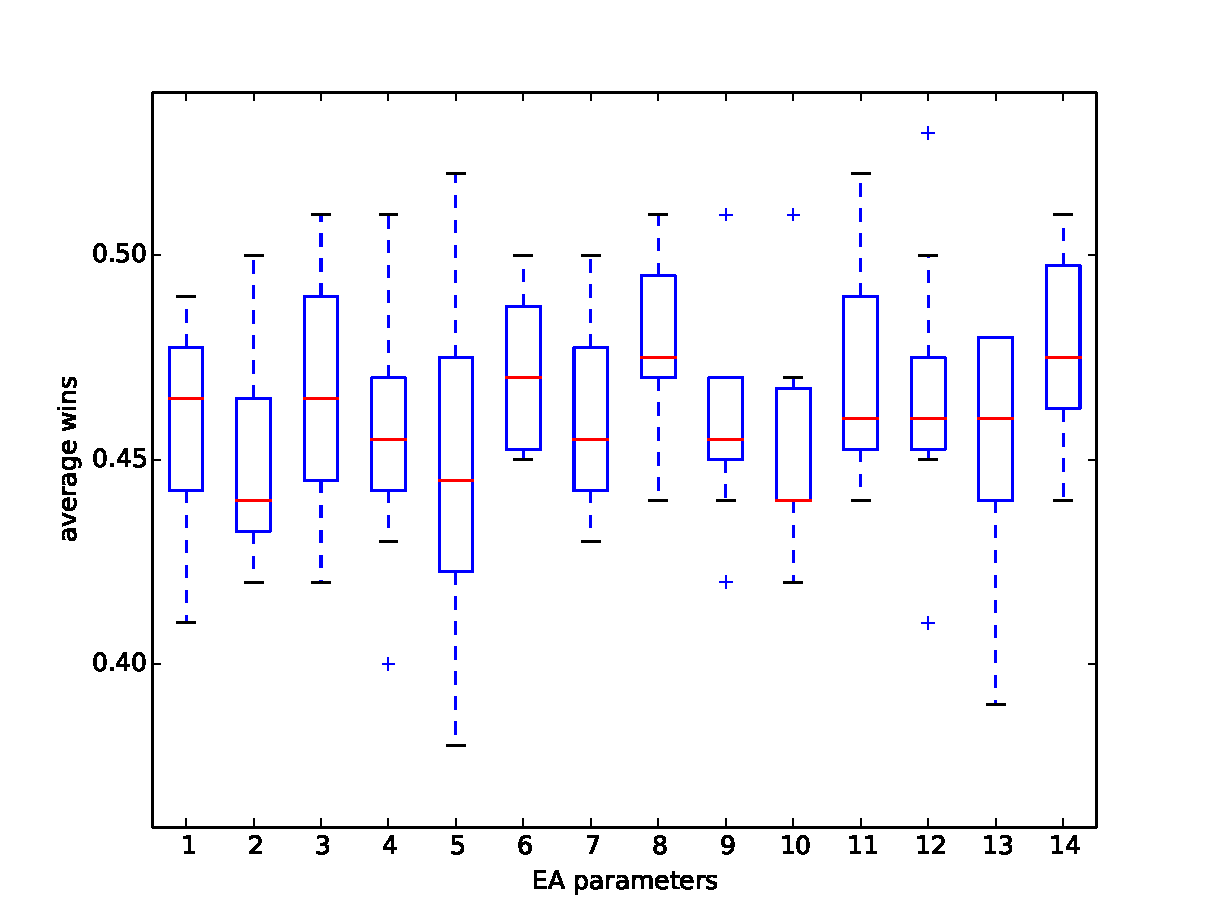
\includegraphics[scale=0.6]{images/eval_evolutionary.pdf}
\caption{boxplot of the \ac{EA} algorithms}
\label{fig:eval_evo}
\end{figure}




\subsection{Evaluation of all approaches} 

Finally we compare the best parameter setups of the three approaches. We defined the best as the agent with the highest average winning rate.
The selected agents are printed bold at each of the result tables.
For a complete comparison there are also the average score and the played time steps evaluated.
The highest winning rate is reached by the heuristic controller (cf.~\cref{all_result}).
But for the highest score we can see that the \ac{MCTS} approaches reaches more points than the others.
For that we can suppose, that the \ac{HR} is playing tighter than the other. This is supported by the least played time steps as well.
Playing tight leads to an earlier win. But there are some games where we could first of all collect points and increase the score and
win at the end.


\begin{table}[H]
\center
\begin{tabular}{*9c}  \hline
\multicolumn{1}{p{1cm}}{\centering approach} & 
\multicolumn{1}{p{1.5cm}}{\centering Avg \\ Wins	} & 
\multicolumn{1}{p{1.5cm}}{\centering Std \\ Wins} &
\multicolumn{1}{p{1.5cm}}{\centering Avg \\ Score	} & 
\multicolumn{1}{p{1.5cm}}{\centering Std \\ Score} &
\multicolumn{1}{p{1.5cm}}{\centering Avg \\ timesteps	} & 
\multicolumn{1}{p{1.5cm}}{\centering Std \\ timesteps} \\ \hline
HR & \textbf{0.532} & 0.027 & 173.7 & 69.39 & \textbf{703.13} & \textbf{19.00} \\ \hline
MCTS & 0.422 & 0.033 & \textbf{222.92} & 63.30 & 1033.01 & 41.20 \\ \hline
EA & 0.479 & \textbf{0.021} & 168.82 & \textbf{42.20} & 827.96 & 42.61 \\ \hline
\end{tabular}
\label{all_result}
\caption{results of all algorithms}
\end{table}

By looking at the boxsplit of the winning rate (cf.~\cref{all_result})



\begin{figure}
\begin{minipage}{.5\textwidth}
\centering
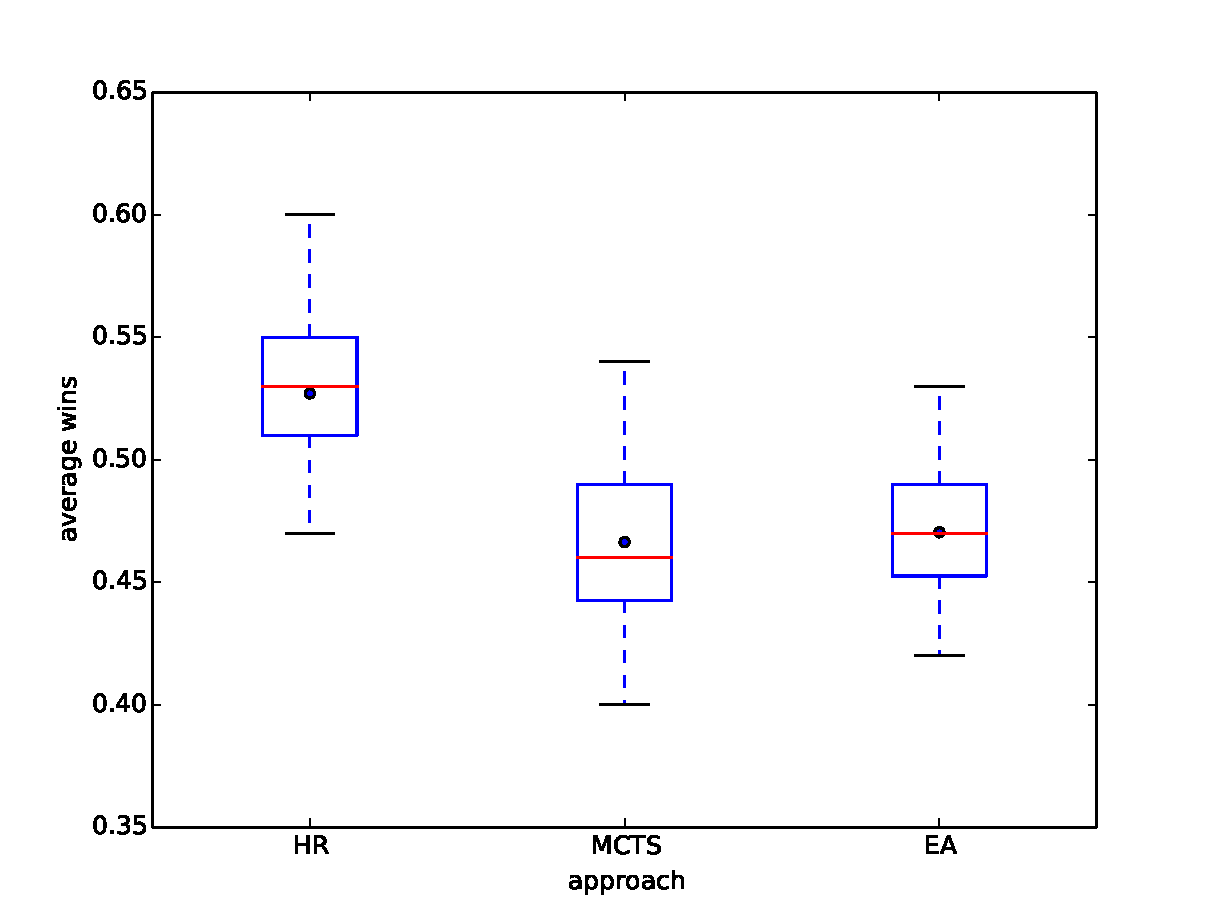
\includegraphics[scale=0.3]{images/eval_all_wins.pdf}
\caption{boxplot of wins}
\label{fig:eval_all_wins}
\end{minipage}%
\begin{minipage}{.5\textwidth}
\centering
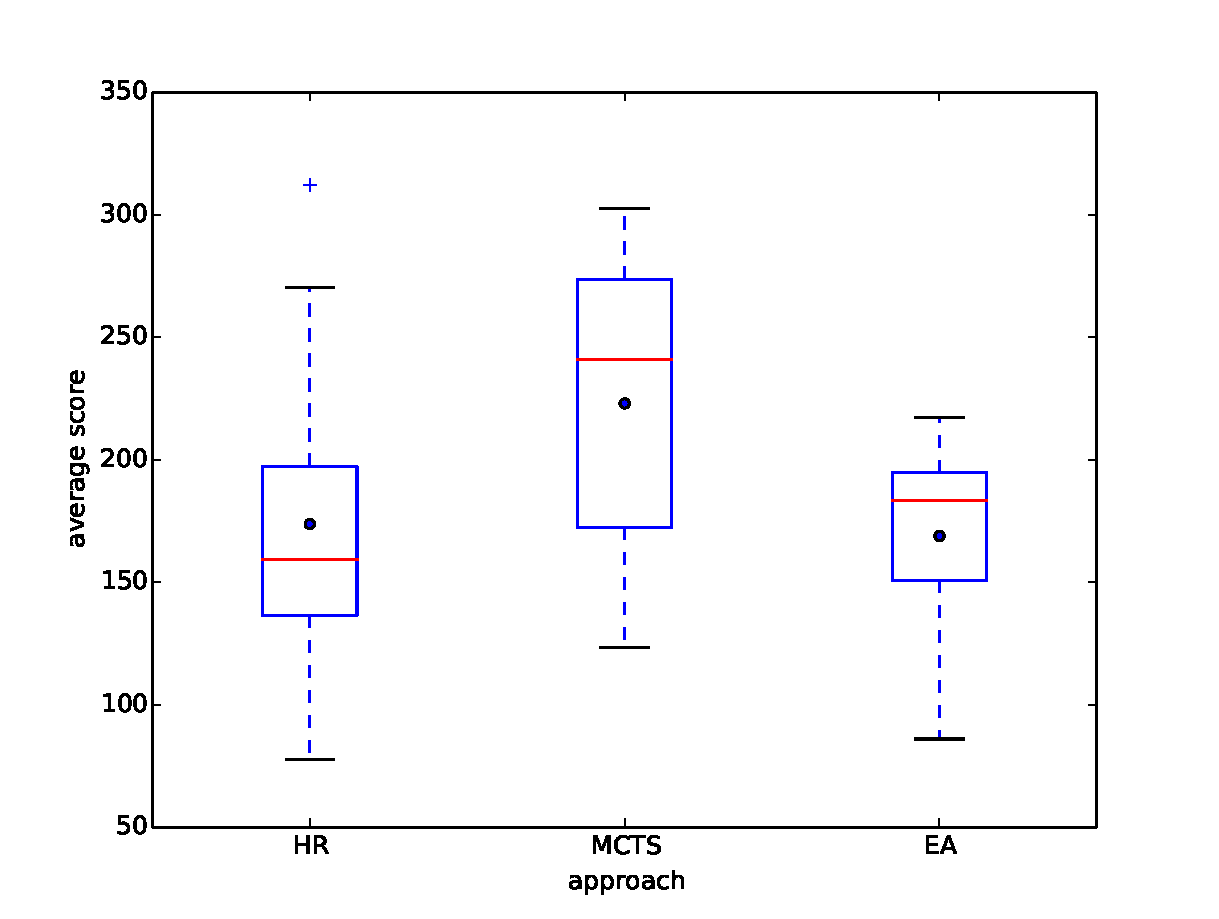
\includegraphics[scale=0.3]{images/eval_all_score.pdf}
\caption{boxplot of score}
\label{fig:eval_all_score}
\end{minipage}
\end{figure}




\begin{figure}[H]
\centering
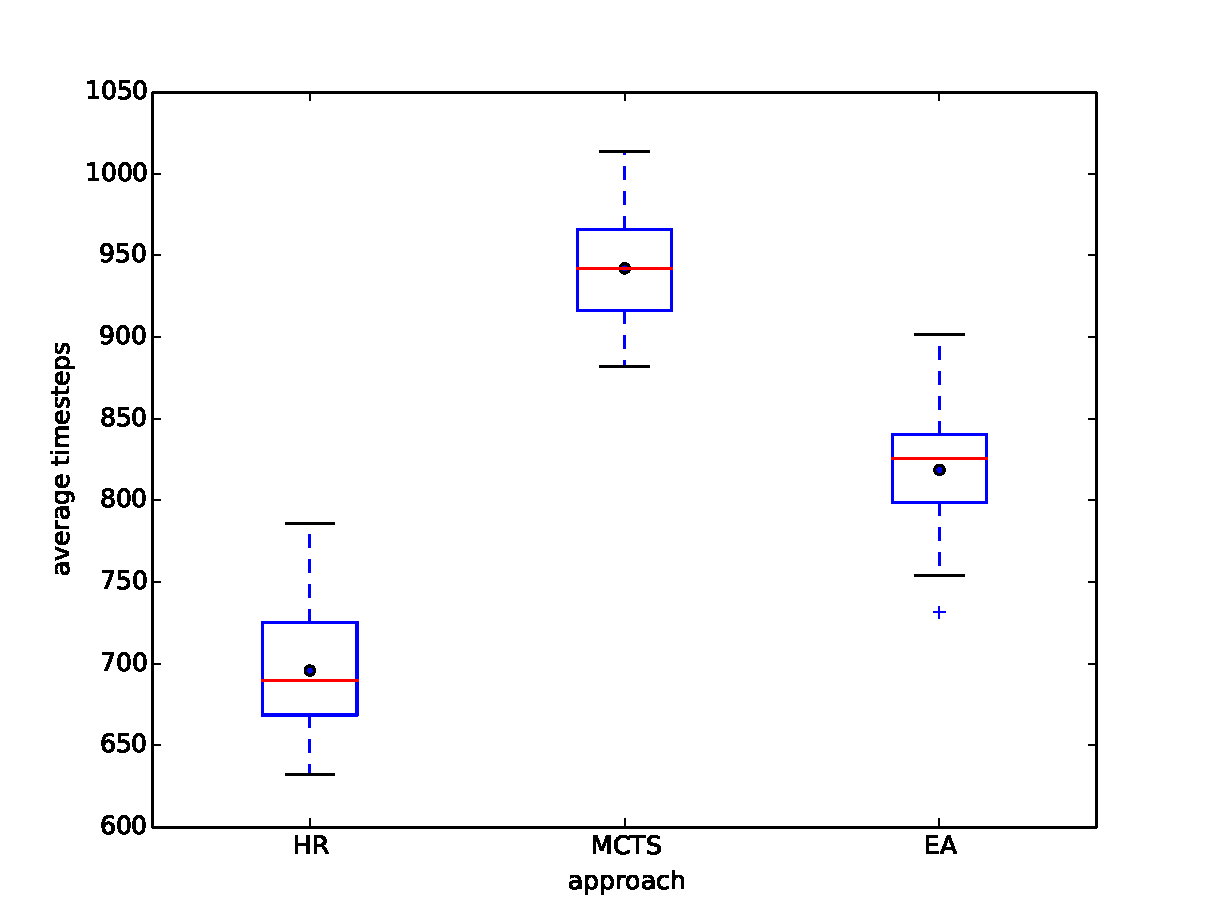
\includegraphics[scale=0.3]{images/eval_all_timesteps.pdf}
\caption{boxplot of timesteps}
\label{fig:eval_all_timesteps}
\end{figure}


\section{Conclusions and Future Work} 
\label{sec:conc}

This paper presents a comparison of several approaches to play general video games. We selected for each research area (\ac{HR}, \ac{RL}, \ac{NI})
one algorithm and implemented that. 


For the evaluation we have to look at the data for example average wins, score and time steps.
We ignored the in-game behaviour of our agents completely and only looked at the statistics. 
Furthermore we were limited by time and computational power which restricts the iterations of our experiment. 
To get more significant results, a experimental setup with more than 1000 iterations (like 3000 in the comparison between the best agents) have to be set up.
Some future work could be to set this setup up and to test the algorithms with more computing power.  
The \ac{HR} approach has the best results (depending on the number of wins) and was better than the \ac{NI} and \ac{MCTS}. This might have several reasons. Firstly our implementation of \ac{MCTS} and \ac{NI} is maybe not very effective or we did not find the optimal parameters to fit our problem. The parameter problem, which depends on the lack of computing power, could be solved with a more powerful machine and a loop over a set of possible parameter-combinations.
Another reason why the \ac{HR} agent wins is that often there are only very few winning-sprites in the game which makes it hard for \ac{MCTS} and \ac{NI} to get a reward and win the game. These games are easy for the heuristic controller. The average score of the \ac{MCTS} controller is higher because the \ac{HR} controller wins very fast without collecting some extra points. 
We can not make general statements about the accuracy of the approaches (\acs{HR}, \acs{RL}, \acs{NI}) using our controllers as quality criterion, but we can say that all of them are useful for \ac{GVGP}.
For future work the implementation of other controllers and methods (e.g. Neuronal Nets, Pheromone) to compare them with the the actual ones would be an idea. Furthermore a test with unknown games would be good, to compare the agents and the methods on completely unknown games.
Another idea for future work is to combine the best properties of the three agents and and create a combined agent.


\newpage

\section*{Acronyms}
\begin{acronym}[YTM]
\setlength{\itemsep}{-\parsep}
\acro{AI}{Artificial Intelligence}
\acro{EA}{Evolutionary Algorithm}
\acro{HR}{Heuristic}
\acro{MDP}{Markov Decision Process}
\acro{MCTS}{Monte Carlo Tree Search}
\acro{NI}{Nature Inspired}
\acro{RL}{Reinforcement Learning}
\acro{TLU}{Threshold Logic Unit}
\acro{UCT}{Upper Confidence Bound}
\acro{CIG}{Computational Intelligence in Games}
\acro{GVGP}{General Video Game Playing}
\end{acronym}



\bibliographystyle{IEEEtranS}
\bibliography{IEEEabrv,literature}

\end{document} 